\begin{tikzpicture}[align=center, arrow/.style={thick, line cap=round, -{Latex[length=1.5mm]}}, font=\footnotesize]
    \matrix[inner sep=0pt, column sep=2em, row sep=0pt] (mtx) {
        \node[inner sep=0pt] (step1) {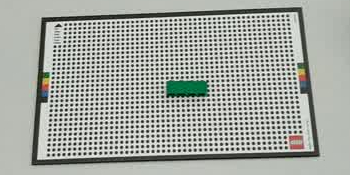
\includegraphics[height=.13\textheight]{img/lego/img1.jpeg}};
        & \node[inner sep=2mm, text width=7em, draw, rectangle, very thick] 
        (instruction) {``Put the white 1x1 brick on top of the green 1x4 brick.''};
        & \node[inner sep=0pt] (step2) {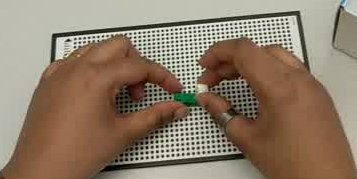
\includegraphics[height=.13\textheight]{img/lego/img2.jpeg}};
        & \node[inner sep=0pt] (step3) {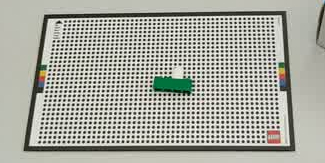
\includegraphics[height=.13\textheight]{img/lego/img3.jpeg}};\\
    };

    \begin{scope}[arrow]
        \draw (step1) -- (instruction);
        \draw (instruction) -- (step2);
        \draw (step2) -- (step3);
    \end{scope}
\end{tikzpicture}